\section{Register description}
\regover{
{\hyperref[2ddma-DMA2D-IntStatus]{DMA2D\_IntStatus}}&
\\
\hline
{\hyperref[2ddma-DMA2D-IntTCStatus]{DMA2D\_IntTCStatus}}&
\\
\hline
{\hyperref[2ddma-DMA2D-IntTCClear]{DMA2D\_IntTCClear}}&
\\
\hline
{\hyperref[2ddma-DMA2D-EnbldChns]{DMA2D\_EnbldChns}}&
\\
\hline
{\hyperref[2ddma-DMA2D-Config]{DMA2D\_Config}}&
\\
\hline
{\hyperref[2ddma-DMA2D-Sync]{DMA2D\_Sync}}&
\\
\hline
{\hyperref[2ddma-DMA2D-SoftBReq]{DMA2D\_SoftBReq}}&
\\
\hline
{\hyperref[2ddma-DMA2D-SoftLBReq]{DMA2D\_SoftLBReq}}&
\\
\hline
{\hyperref[2ddma-DMA2D-SoftSReq]{DMA2D\_SoftSReq}}&
\\
\hline
{\hyperref[2ddma-DMA2D-SoftLSReq]{DMA2D\_SoftLSReq}}&
\\
\hline
{\hyperref[2ddma-DMA2D-C0SrcAddr]{DMA2D\_C0SrcAddr}}&
\\
\hline
{\hyperref[2ddma-DMA2D-C0DstAddr]{DMA2D\_C0DstAddr}}&
\\
\hline
{\hyperref[2ddma-DMA2D-C0LLI]{DMA2D\_C0LLI}}&
\\
\hline
{\hyperref[2ddma-DMA2D-C0-BUS]{DMA2D\_C0\_BUS}}&
\\
\hline
{\hyperref[2ddma-DMA2D-C0-SRC-CNT]{DMA2D\_C0\_SRC\_CNT}}&
\\
\hline
{\hyperref[2ddma-DMA2D-C0-SRC-XIC]{DMA2D\_C0\_SRC\_XIC}}&
\\
\hline
{\hyperref[2ddma-DMA2D-C0-SRC-YIC]{DMA2D\_C0\_SRC\_YIC}}&
\\
\hline
{\hyperref[2ddma-DMA2D-C0-DST-CNT]{DMA2D\_C0\_DST\_CNT}}&
\\
\hline
{\hyperref[2ddma-DMA2D-C0-DST-XIC]{DMA2D\_C0\_DST\_XIC}}&
\\
\hline
{\hyperref[2ddma-DMA2D-C0-DST-YIC]{DMA2D\_C0\_DST\_YIC}}&
\\
\hline
{\hyperref[2ddma-DMA2D-C0-KEY]{DMA2D\_C0\_KEY}}&
\\
\hline
{\hyperref[2ddma-DMA2D-C0-KEY-EN]{DMA2D\_C0\_KEY\_EN}}&
\\
\hline
{\hyperref[2ddma-DMA2D-C0-CFG]{DMA2D\_C0\_CFG}}&
\\
\hline
}

\subsection{DMA2D\_IntStatus}
\label{2ddma-DMA2D-IntStatus}
Address:0x30006000
 \begin{figure}[H]
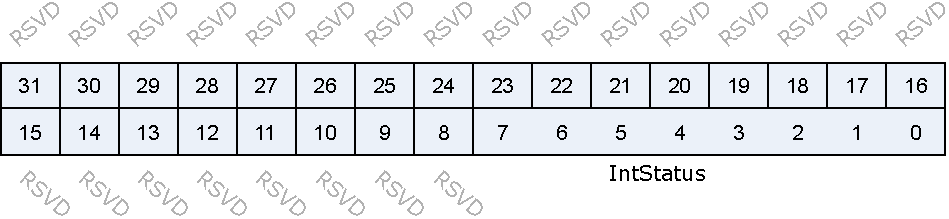
\includegraphics{2ddma_DMA2D_IntStatus.pdf}
\end{figure}

\regdes{31:8&RSVD& & & \\\hline
7:0&IntStatus&r&0&Status of the DMA interrupts after masking\\\hline

}
\subsection{DMA2D\_IntTCStatus}
\label{2ddma-DMA2D-IntTCStatus}
Address:0x30006004
 \begin{figure}[H]
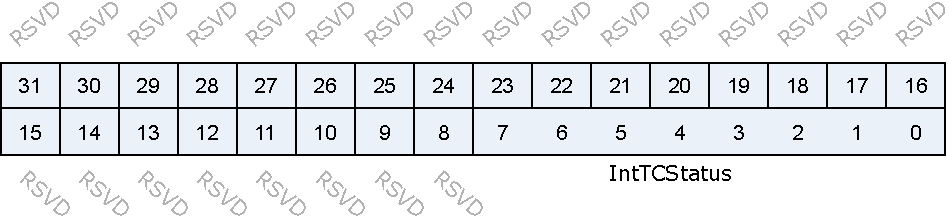
\includegraphics{2ddma_DMA2D_IntTCStatus.pdf}
\end{figure}

\regdes{31:8&RSVD& & & \\\hline
7:0&IntTCStatus&r&0&Interrupt terminal count request status\\\hline

}
\subsection{DMA2D\_IntTCClear}
\label{2ddma-DMA2D-IntTCClear}
Address:0x30006008
 \begin{figure}[H]
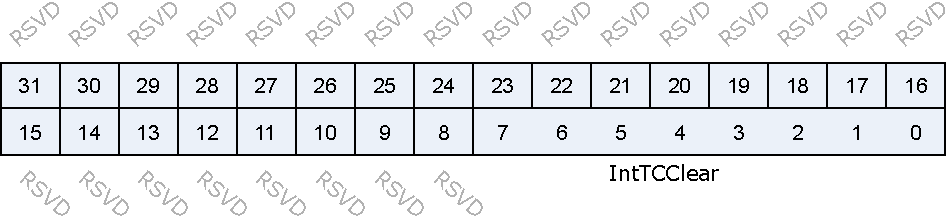
\includegraphics{2ddma_DMA2D_IntTCClear.pdf}
\end{figure}

\regdes{31:8&RSVD& & & \\\hline
7:0&IntTCClear&w1p&0&Terminal count request clear\\\hline

}
\subsection{DMA2D\_EnbldChns}
\label{2ddma-DMA2D-EnbldChns}
Address:0x3000600c
 \begin{figure}[H]
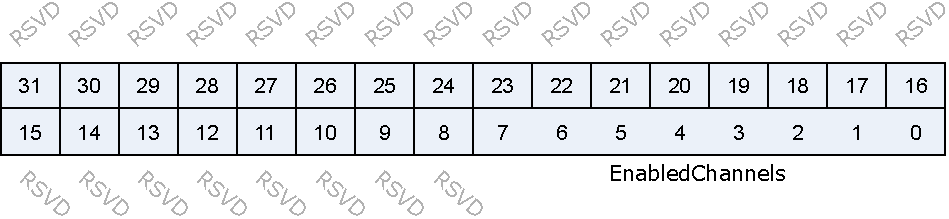
\includegraphics{2ddma_DMA2D_EnbldChns.pdf}
\end{figure}

\regdes{31:8&RSVD& & & \\\hline
7:0&EnabledChannels&r&0&Channel enable status\\\hline

}
\subsection{DMA2D\_Config}
\label{2ddma-DMA2D-Config}
Address:0x30006010
 \begin{figure}[H]
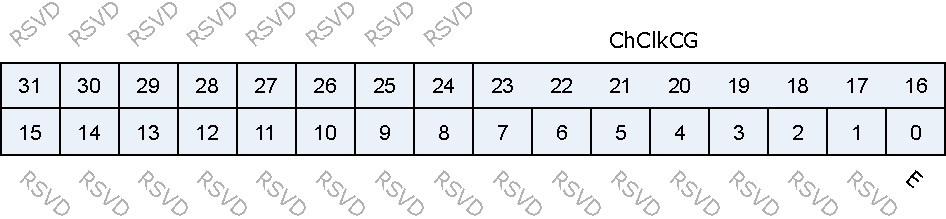
\includegraphics{2ddma_DMA2D_Config.pdf}
\end{figure}

\regdes{31:24&RSVD& & & \\\hline
23:16&ChClkCG&r/w&8'hff&Channel Clock cg enable\\\hline
15:1&RSVD& & & \\\hline
0&E&r/w&0&SMDMA Enable.\\\hline

}
\subsection{DMA2D\_Sync}
\label{2ddma-DMA2D-Sync}
Address:0x30006014
 \begin{figure}[H]
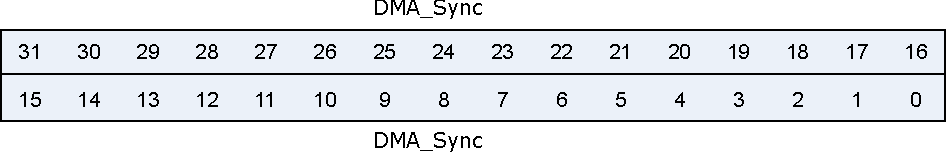
\includegraphics{2ddma_DMA2D_Sync.pdf}
\end{figure}

\regdes{31:0&DMA\_Sync&r/w&0&DMA synchronization logic for DMA request signals: 0 = enable, 1 = disable\\\hline

}
\subsection{DMA2D\_SoftBReq}
\label{2ddma-DMA2D-SoftBReq}
Address:0x30006018
 \begin{figure}[H]
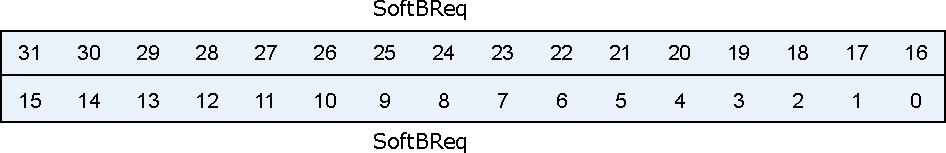
\includegraphics{2ddma_DMA2D_SoftBReq.pdf}
\end{figure}

\regdes{31:0&SoftBReq&r/w&0&Software burst request\\\hline

}
\subsection{DMA2D\_SoftLBReq}
\label{2ddma-DMA2D-SoftLBReq}
Address:0x3000601c
 \begin{figure}[H]
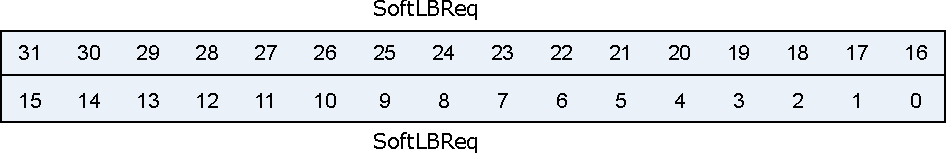
\includegraphics{2ddma_DMA2D_SoftLBReq.pdf}
\end{figure}

\regdes{31:0&SoftLBReq&r/w&0&Software last burst request\\\hline

}
\subsection{DMA2D\_SoftSReq}
\label{2ddma-DMA2D-SoftSReq}
Address:0x30006020
 \begin{figure}[H]
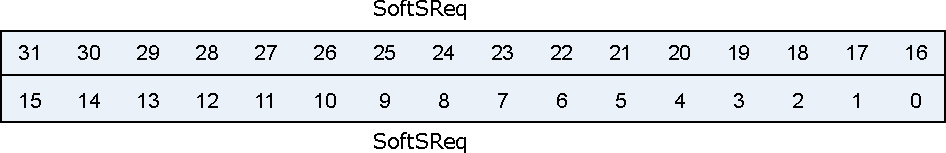
\includegraphics{2ddma_DMA2D_SoftSReq.pdf}
\end{figure}

\regdes{31:0&SoftSReq&r/w&0&Software signle request\\\hline

}
\subsection{DMA2D\_SoftLSReq}
\label{2ddma-DMA2D-SoftLSReq}
Address:0x30006024
 \begin{figure}[H]
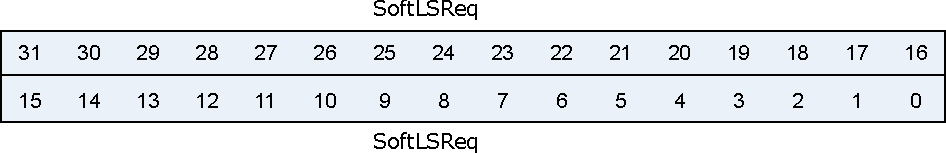
\includegraphics{2ddma_DMA2D_SoftLSReq.pdf}
\end{figure}

\regdes{31:0&SoftLSReq&r/w&0&Software last signle request\\\hline

}
\subsection{DMA2D\_C0SrcAddr}
\label{2ddma-DMA2D-C0SrcAddr}
Address:0x30006100
 \begin{figure}[H]
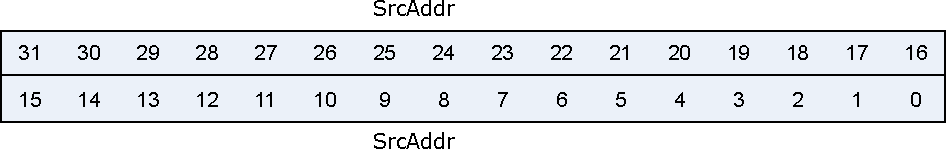
\includegraphics{2ddma_DMA2D_C0SrcAddr.pdf}
\end{figure}

\regdes{31:0&SrcAddr&r/w&0&DMA source address\\\hline

}
\subsection{DMA2D\_C0DstAddr}
\label{2ddma-DMA2D-C0DstAddr}
Address:0x30006104
 \begin{figure}[H]
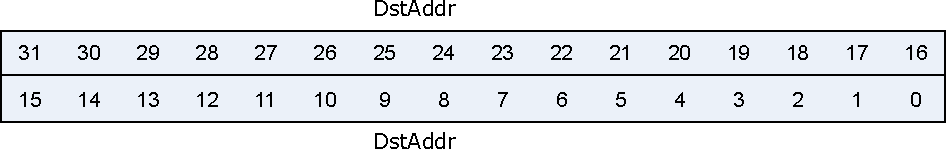
\includegraphics{2ddma_DMA2D_C0DstAddr.pdf}
\end{figure}

\regdes{31:0&DstAddr&r/w&0&DMA Destination address\\\hline

}
\subsection{DMA2D\_C0LLI}
\label{2ddma-DMA2D-C0LLI}
Address:0x30006108
 \begin{figure}[H]
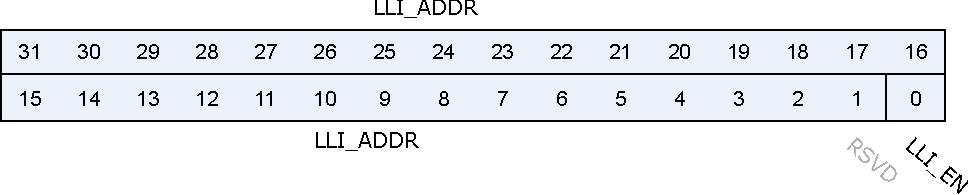
\includegraphics{2ddma_DMA2D_C0LLI.pdf}
\end{figure}

\regdes{31:2&LLI\_ADDR&r/w&0&Next linked list address\\\hline
1&RSVD& & & \\\hline
0&LLI\_EN&r/w&0&Next LLI enable\\\hline

}
\subsection{DMA2D\_C0\_BUS}
\label{2ddma-DMA2D-C0-BUS}
Address:0x3000610c
 \begin{figure}[H]
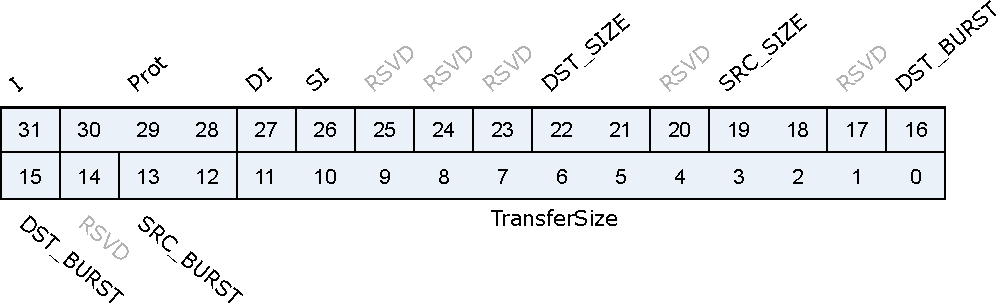
\includegraphics{2ddma_DMA2D_C0_BUS.pdf}
\end{figure}

\regdes{31&I&r/w&0&Terminal count interrupt enable bit. It controls whether the current LLI is expected to trigger the terminal count interrupt.\\\hline
30:28&Prot&r/w&0&Hprot Setting\\\hline
27&DI&r/w&1&Only work when reg\_dma\_2d\_en = 0 \par Destination increment. When set, the Destination address is incremented after each transfer.
\\\hline
26&SI&r/w&1&Only work when reg\_dma\_2d\_en = 0 \par Source increment. When set, the source address is incremented after each transfer.
\\\hline
25:23&RSVD& & & \\\hline
22:21&DST\_SIZE&r/w&2'd2&Destination transfer width: 8/16/32\\\hline
20&RSVD& & & \\\hline
19:18&SRC\_SIZE&r/w&2'd2&Source transfer width: 8/16/32\\\hline
17&RSVD& & & \\\hline
16:15&DST\_BURST&r/w&2'd1&Destination burst size: 1/4/8/16\\\hline
14&RSVD& & & \\\hline
13:12&SRC\_BURST&r/w&2'd1&\\\hline
11:0&TransferSize&r/w&0&Only work when reg\_dma\_2d\_en = 0 \par Transfer size: 0~4095. Number of data transfers left to complete when the SMDMA is the flow controller.
\\\hline

}
\subsection{DMA2D\_C0\_SRC\_CNT}
\label{2ddma-DMA2D-C0-SRC-CNT}
Address:0x30006110
 \begin{figure}[H]
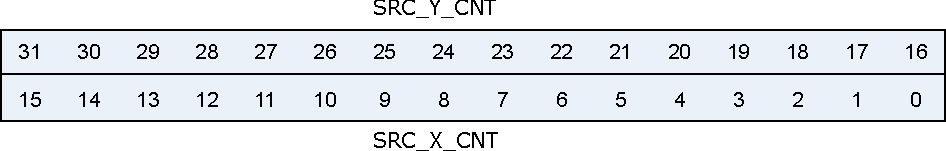
\includegraphics{2ddma_DMA2D_C0_SRC_CNT.pdf}
\end{figure}

\regdes{31:16&SRC\_Y\_CNT&r/w&16'd0&Only work when reg\_dma\_2d\_en = 1 \par Source Y-direction Count
\\\hline
15:0&SRC\_X\_CNT&r/w&16'd0&Only work when reg\_dma\_2d\_en = 1 \par Source X-direction Count
\\\hline

}
\subsection{DMA2D\_C0\_SRC\_XIC}
\label{2ddma-DMA2D-C0-SRC-XIC}
Address:0x30006114
 \begin{figure}[H]
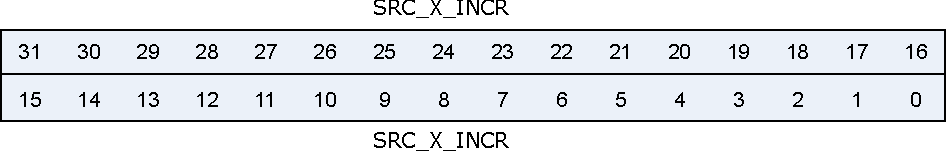
\includegraphics{2ddma_DMA2D_C0_SRC_XIC.pdf}
\end{figure}

\regdes{31:0&SRC\_X\_INCR&r/w&32'd0&Only work when reg\_dma\_2d\_en = 1 \par Source Y-direction address increment \par Must allign "SWidth" setting \par [16] sign-bit
\\\hline

}
\subsection{DMA2D\_C0\_SRC\_YIC}
\label{2ddma-DMA2D-C0-SRC-YIC}
Address:0x30006118
 \begin{figure}[H]
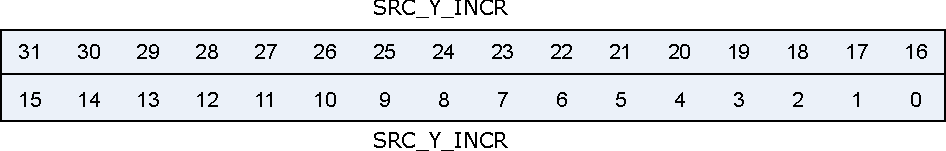
\includegraphics{2ddma_DMA2D_C0_SRC_YIC.pdf}
\end{figure}

\regdes{31:0&SRC\_Y\_INCR&r/w&32'd0&Only work when reg\_dma\_2d\_en = 1 \par Source Y-direction address increment \par Must allign "SWidth" setting \par [16] sign-bit
\\\hline

}
\subsection{DMA2D\_C0\_DST\_CNT}
\label{2ddma-DMA2D-C0-DST-CNT}
Address:0x3000611c
 \begin{figure}[H]
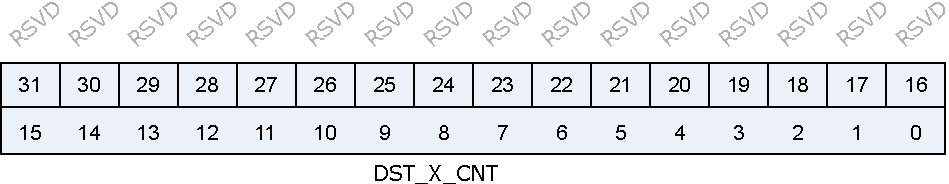
\includegraphics{2ddma_DMA2D_C0_DST_CNT.pdf}
\end{figure}

\regdes{31:16&RSVD& & & \\\hline
15:0&DST\_X\_CNT&r/w&16'd0&Only work when reg\_dma\_2d\_en = 1 \par Source X-direction Count
\\\hline

}
\subsection{DMA2D\_C0\_DST\_XIC}
\label{2ddma-DMA2D-C0-DST-XIC}
Address:0x30006120
 \begin{figure}[H]
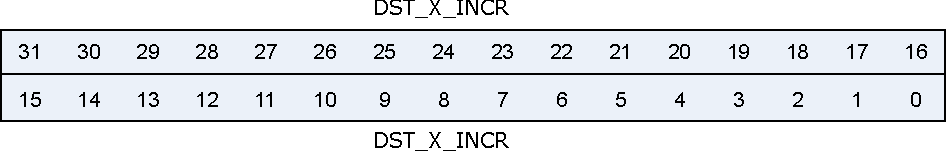
\includegraphics{2ddma_DMA2D_C0_DST_XIC.pdf}
\end{figure}

\regdes{31:0&DST\_X\_INCR&r/w&32'd0&Only work when reg\_dma\_2d\_en = 1 \par Source Y-direction address increment \par Must allign "SWidth" setting \par [16] sign-bit
\\\hline

}
\subsection{DMA2D\_C0\_DST\_YIC}
\label{2ddma-DMA2D-C0-DST-YIC}
Address:0x30006124
 \begin{figure}[H]
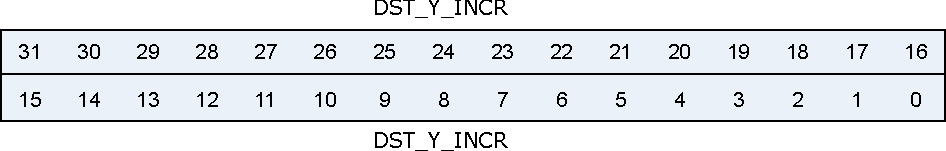
\includegraphics{2ddma_DMA2D_C0_DST_YIC.pdf}
\end{figure}

\regdes{31:0&DST\_Y\_INCR&r/w&32'd0&Only work when reg\_dma\_2d\_en = 1 \par Desitination Y-direction address increment \par Must allign "DWidth" setting \par [16] sign-bit
\\\hline

}
\subsection{DMA2D\_C0\_KEY}
\label{2ddma-DMA2D-C0-KEY}
Address:0x30006174
 \begin{figure}[H]
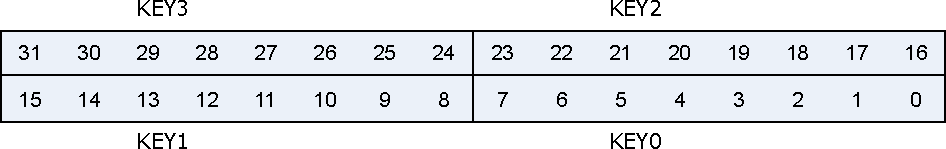
\includegraphics{2ddma_DMA2D_C0_KEY.pdf}
\end{figure}

\regdes{31:24&KEY3&r/w&0&Key value\\\hline
23:16&KEY2&r/w&0&Key value\\\hline
15:8&KEY1&r/w&0&Key value\\\hline
7:0&KEY0&r/w&0&Key value\\\hline

}
\subsection{DMA2D\_C0\_KEY\_EN}
\label{2ddma-DMA2D-C0-KEY-EN}
Address:0x30006178
 \begin{figure}[H]
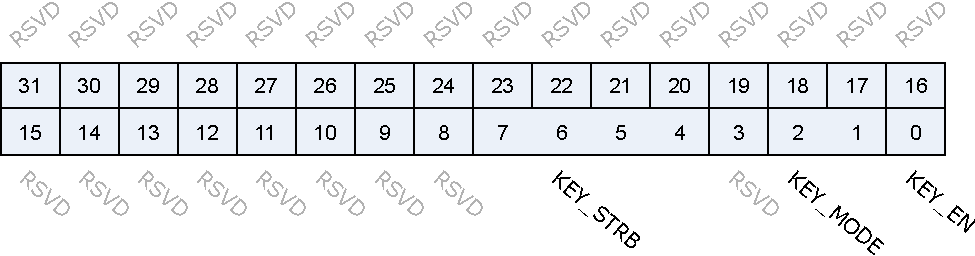
\includegraphics{2ddma_DMA2D_C0_KEY_EN.pdf}
\end{figure}

\regdes{31:8&RSVD& & & \\\hline
7:4&KEY\_STRB&r/w&4'h0&According Key mode set Key STRB \par Key mode : Key STRB \par 2'd0 : 4'h1 \par 2'd1 : 4'h3 \par 2'd2 : 4'h7 \par 2'd3 : 4'hf
\\\hline
3&RSVD& & & \\\hline
2:1&KEY\_MODE&r/w&0&Key Mode \par 2'd0 : 8-bit mode \par 2'd1 : 16-bit mode \par 2'd2 : 24-bit mode \par 2'd3 : 32-bit mode
\\\hline
0&KEY\_EN&r/w&0&Key enable\\\hline

}
\subsection{DMA2D\_C0\_CFG}
\label{2ddma-DMA2D-C0-CFG}
Address:0x3000617c
 \begin{figure}[H]
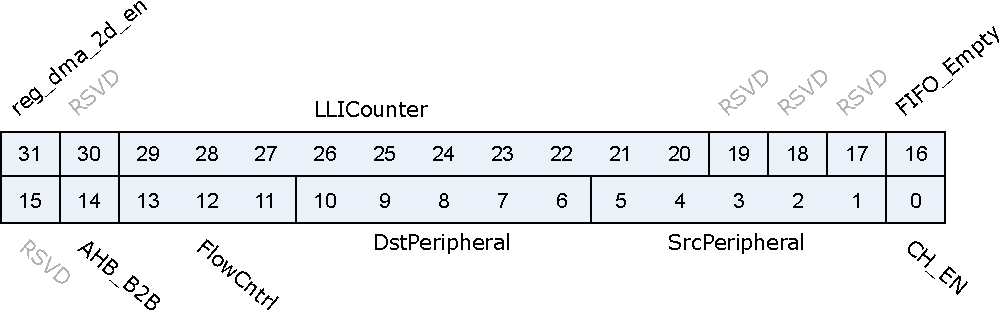
\includegraphics{2ddma_DMA2D_C0_CFG.pdf}
\end{figure}

\regdes{31&reg\_dma\_2d\_en&r/w&0&DMA 2d enable\\\hline
30&RSVD& & & \\\hline
29:20&LLICounter&r&0&LLI counter. Increased 1 each LLI run. Cleared 0 when config Control.\\\hline
19:17&RSVD& & & \\\hline
16&FIFO\_Empty&r&0&Active: 0 = no data in FIFO of the channel, 1 = FIFO of the channel has data.\\\hline
15&RSVD& & & \\\hline
14&AHB\_B2B&r/w&0&AHB back to back enable\\\hline
13:11&FlowCntrl&r/w&0&000: Memory-to-memory (DMA) \par 001: Memory-to-peripheral (DMA) \par 010: Peripheral-to-memory (DMA) \par 011: Source peripheral-to-Destination peripheral (DMA) \par The following only work when reg\_dma\_2d\_en=0 :  \par 100: Source peripheral-to-Destination peripheral (Destination peripheral) \par 101: Memory-to-peripheral (peripheral) \par 110: Peripheral-to-memory (peripheral) \par 111: Source peripheral-to-Destination peripheral (Source peripheral)
\\\hline
10:6&DstPeripheral&r/w&0&Destination peripheral.\\\hline
5:1&SrcPeripheral&r/w&0&Source peripheral.\\\hline
0&CH\_EN&r/w&0&Channel enable.\\\hline

}
